% Options for packages loaded elsewhere
\PassOptionsToPackage{unicode}{hyperref}
\PassOptionsToPackage{hyphens}{url}
%
\documentclass[
]{article}
\usepackage{amsmath,amssymb}
\usepackage{lmodern}
\usepackage{iftex}
\ifPDFTeX
  \usepackage[T1]{fontenc}
  \usepackage[utf8]{inputenc}
  \usepackage{textcomp} % provide euro and other symbols
\else % if luatex or xetex
  \usepackage{unicode-math}
  \defaultfontfeatures{Scale=MatchLowercase}
  \defaultfontfeatures[\rmfamily]{Ligatures=TeX,Scale=1}
\fi
% Use upquote if available, for straight quotes in verbatim environments
\IfFileExists{upquote.sty}{\usepackage{upquote}}{}
\IfFileExists{microtype.sty}{% use microtype if available
  \usepackage[]{microtype}
  \UseMicrotypeSet[protrusion]{basicmath} % disable protrusion for tt fonts
}{}
\makeatletter
\@ifundefined{KOMAClassName}{% if non-KOMA class
  \IfFileExists{parskip.sty}{%
    \usepackage{parskip}
  }{% else
    \setlength{\parindent}{0pt}
    \setlength{\parskip}{6pt plus 2pt minus 1pt}}
}{% if KOMA class
  \KOMAoptions{parskip=half}}
\makeatother
\usepackage{xcolor}
\IfFileExists{xurl.sty}{\usepackage{xurl}}{} % add URL line breaks if available
\IfFileExists{bookmark.sty}{\usepackage{bookmark}}{\usepackage{hyperref}}
\hypersetup{
  pdftitle={Visual proteomics using whole-lamella 2D template matching},
  pdfauthor={Johannes ElferichNikolaus Grigorieff},
  pdflang={en-US},
  pdfkeywords={cryo-EM, visual protemics, ribosome},
  hidelinks,
  pdfcreator={LaTeX via pandoc}}
\urlstyle{same} % disable monospaced font for URLs
\usepackage{graphicx}
\makeatletter
\def\maxwidth{\ifdim\Gin@nat@width>\linewidth\linewidth\else\Gin@nat@width\fi}
\def\maxheight{\ifdim\Gin@nat@height>\textheight\textheight\else\Gin@nat@height\fi}
\makeatother
% Scale images if necessary, so that they will not overflow the page
% margins by default, and it is still possible to overwrite the defaults
% using explicit options in \includegraphics[width, height, ...]{}
\setkeys{Gin}{width=\maxwidth,height=\maxheight,keepaspectratio}
% Set default figure placement to htbp
\makeatletter
\def\fps@figure{htbp}
\makeatother
\setlength{\emergencystretch}{3em} % prevent overfull lines
\providecommand{\tightlist}{%
  \setlength{\itemsep}{0pt}\setlength{\parskip}{0pt}}
\setcounter{secnumdepth}{-\maxdimen} % remove section numbering
\newlength{\cslhangindent}
\setlength{\cslhangindent}{1.5em}
\newlength{\csllabelwidth}
\setlength{\csllabelwidth}{3em}
\newlength{\cslentryspacingunit} % times entry-spacing
\setlength{\cslentryspacingunit}{\parskip}
\newenvironment{CSLReferences}[2] % #1 hanging-ident, #2 entry spacing
 {% don't indent paragraphs
  \setlength{\parindent}{0pt}
  % turn on hanging indent if param 1 is 1
  \ifodd #1
  \let\oldpar\par
  \def\par{\hangindent=\cslhangindent\oldpar}
  \fi
  % set entry spacing
  \setlength{\parskip}{#2\cslentryspacingunit}
 }%
 {}
\usepackage{calc}
\newcommand{\CSLBlock}[1]{#1\hfill\break}
\newcommand{\CSLLeftMargin}[1]{\parbox[t]{\csllabelwidth}{#1}}
\newcommand{\CSLRightInline}[1]{\parbox[t]{\linewidth - \csllabelwidth}{#1}\break}
\newcommand{\CSLIndent}[1]{\hspace{\cslhangindent}#1}
\ifLuaTeX
\usepackage[bidi=basic]{babel}
\else
\usepackage[bidi=default]{babel}
\fi
\babelprovide[main,import]{american}
% get rid of language-specific shorthands (see #6817):
\let\LanguageShortHands\languageshorthands
\def\languageshorthands#1{}

%%%% pandoc-fignos: required package
\usepackage{caption}

%% pandoc-fignos: environment to disable figure caption prefixes
\makeatletter
\newcounter{figno}
\newenvironment{fignos:no-prefix-figure-caption}{
  \caption@ifcompatibility{}{
    \let\oldthefigure\thefigure
    \let\oldtheHfigure\theHfigure
    \renewcommand{\thefigure}{figno:\thefigno}
    \renewcommand{\theHfigure}{figno:\thefigno}
    \stepcounter{figno}
    \captionsetup{labelformat=empty}
  }
}{
  \caption@ifcompatibility{}{
    \captionsetup{labelformat=default}
    \let\thefigure\oldthefigure
    \let\theHfigure\oldtheHfigure
    \addtocounter{figure}{-1}
  }
}
\makeatother
\ifLuaTeX
  \usepackage{selnolig}  % disable illegal ligatures
\fi

\title{Visual proteomics using whole-lamella 2D template matching}
\author{}
\date{}

\begin{document}
\maketitle

This manuscript
(\href{https://jojoelfe.github.io/fowl_template_matching_manuscript/v/3fd92a26614a26949905aec5a87c6e0dabaffd3a/}{permalink})
was automatically generated
from \href{https://github.com/jojoelfe/fowl_template_matching_manuscript/tree/3fd92a26614a26949905aec5a87c6e0dabaffd3a}{jojoelfe/fowl\_template\_matching\_manuscript@3fd92a2}
on January 4, 2022.

\hypertarget{authors}{%
\subsection{Authors}\label{authors}}

\begin{itemize}
\item
  \textbf{Johannes Elferich}
  
\includegraphics[width=0.16667in,height=0.16667in]{images/orcid.pdf}
  \href{https://orcid.org/XXXX-XXXX-XXXX-XXXX}{XXXX-XXXX-XXXX-XXXX}
  · 
\includegraphics[width=0.16667in,height=0.16667in]{images/github.pdf}
  \href{https://github.com/jojoelfe}{jojoelfe}
  RNA Therapeutic INstitute, UMass Chan Medical SChool; HHMI
\item
  \textbf{Nikolaus Grigorieff}
  
\includegraphics[width=0.16667in,height=0.16667in]{images/orcid.pdf}
  \href{https://orcid.org/XXXX-XXXX-XXXX-XXXX}{XXXX-XXXX-XXXX-XXXX}
  · 
\includegraphics[width=0.16667in,height=0.16667in]{images/github.pdf}
  \href{https://github.com/nikogrigorieff}{nikogrigorieff}
  RNA Therapeutic INstitute, UMass Chan Medical SChool; HHMI
\end{itemize}

\hypertarget{abstract}{%
\subsection{Abstract}\label{abstract}}

Localization and characterization of biomolecules inside a cell is the fundamental quest of all biological imaging. Fluorescence microscopy can localize biomolecules inside whole cells and tissues, but its ability to count biomolecules and accuracy of the spatial coordinates is limited by the wavelength of visible light. Cryo-electron microscopy on the other hand provides highly accurate position and orientation information of biomolecules but is often limited to small fields of view inside a cell, providing only limited biological context. In this study we use a data-acquisition scheme called ``Fast Observation of Whole Lamella'' (FOWL) to collect cryo-electron microscopy data over thin central sections, representing roughly 1\% of the total cellular volume, of neutrophil-like mouse cells. We use 2D-template matching to determine localization and orientation of the large subunit of the ribosome in these cross-sections. We furthermore use 2D-template matching to test for complex formation with the small ribosomal subunit and used relative orientations of ribosome to assign ribosomes to polysomes. Overall these results provide a ``map'' of translational activity in cross-sections of mammalian cells. We envision that using these high-throughput cryo-EM data collection and 2D template matching approaches will advance visual proteomics to complement other single-cell ``omics'' techniques, such as flow-cytometry and single-cell sequencing.

\hypertarget{introduction}{%
\subsection{Introduction}\label{introduction}}

Understanding of cellular processes requires knowledge of the amount, location, and interaction of biomolecules inside the cell. Techniques that measure this can broadly be divided into label, and label-free techniques. In label-techniques a probe is physically attahced to a molecule is interest that is able to produce a high signal-to-noise signal, such as a fluorescent probe. In label-free techniques the physical properties of molecules themselves are used for detection. An example for this is proteomics using mass-spectrometry. Broadly the advantage of label-free techniques is that they can provide information over thousands of molecules, while label-techniques offer higher fidelity information for a few molecules. Especially spatial information can most of the time only be achieved using label-tehcniques.

Cryo-electron microscopy has the potential to directly measure the arrangement of atoms that compose biomolecules inside of cells, therby allowing label-free detection with high spatial accuracy. This has been called ``Visual proteomics''. The predominant technique at the moemnt is cryo-electron tomography. However, the throughput of these methods in low due to highly complex sample preparation, data acquisition, and data processing. We have shown that molecules can be identified by their structural ``fingerprint'' in single projection using ``2D temaplte-matching''.

Here we apply 2D-template matching to neutrophil-ilke murine cells. By employing anew data-acquisition scheme we obtained coverage of the whole ``lamella'' covering roughly 2\% of the cellular volume.

\hypertarget{materials-and-methods}{%
\subsection{Materials and Methods}\label{materials-and-methods}}

\hypertarget{grid-preparation}{%
\subsubsection{Grid preparation}\label{grid-preparation}}

ER-HoxA9 cells were maintained in RPMI supplemented with 10\% FBS, penicillin/streptomycin, SCF, and estrogen {[}\protect\hyperlink{ref-1B9Vt9eYu}{1}{]} at 37C and 5\% CO2. 120h prior to gridd freezing cells were washed twice in PBS and cultured in the same medium, except without estrogen. Differentiation was verified by staining with Hoechst-dye and insepction of nuclear morphology. Cells were then counted and diluted to 1\^{}106 cells/ml. Grids ( either 200 mesh copper grids, with a sillicone-oxide and 2um holes with a 2um spacing or 200 mesh gold grids with a thin gold film and 2 um holes in 2um sapcing) were glow-discharged from both sides using a \ldots{} for \ldots{} . 3.5 ul of cells suspension was added to grids on the thin-film side and grids were automatically blotted from the back-side using a GP2 cryoplunger (Leica) for \ldots{} s and rapidly plunged into liquid ethane at -185C.

\hypertarget{fib-milling}{%
\subsubsection{FIB-milling}\label{fib-milling}}

Grids were loaded into a Acquilos 2 FIB/SEM microscope with a stage cooled to -190C. Grids were sputter-coated with platinum for 15s at 45 mA and then coated with a layer of platinum-precursor by openin the GIS-valve for 45s. An overview of the grid was created by montaging SEM images and isolated cells at the center of gridsquares were selected for FB-milling. Lamella were generated automatically using the AutoTEM software, resulting in 6-8 um wide lamella with 150-200 um thickness as determined by FIB-imaging of the lamella edge.

\hypertarget{data-collection}{%
\subsubsection{Data collection}\label{data-collection}}

Grids were loaded into a Krios Titam TEM operated at 300 keV. The microscope was setup with a cross-grating grid on the stageby setting the beam-diameter to 900 nm, resulting in the beam being completely visible in the camera. To establish fringe-free conditions, the ``Fine eucentric'' procedure of serialEM was used to move a square of the cross-grating grid to the eucentric position of the microscope. The effective defocus was then set to 2 um, using the ``autofocus'' routine of serialEM. The objective focus of the microscope was changed until no fringes were visible. The stage was then moved in Z until images had a apparent defocus of 2 um. The differnce in stage Z-position between the eucentric and fringe-free conditions was calculate d and noted to move other areas into fringe-free condition.

Low magnification montages were used to find lamella and lamella that were sufficently thin and free of contamination were selected for automated data collection.

\hypertarget{data-pre-processing}{%
\subsubsection{Data pre-processing}\label{data-pre-processing}}

\hypertarget{template-matching}{%
\subsubsection{Template matching}\label{template-matching}}

\hypertarget{data-analysis}{%
\subsubsection{Data analysis}\label{data-analysis}}

\hypertarget{introduction-1}{%
\subsection{Introduction}\label{introduction-1}}

\hypertarget{introduction-2}{%
\subsection{Introduction}\label{introduction-2}}

\hypertarget{figures}{%
\subsection{Figures}\label{figures}}

\begin{fignos:no-prefix-figure-caption}

\begin{figure}
\centering
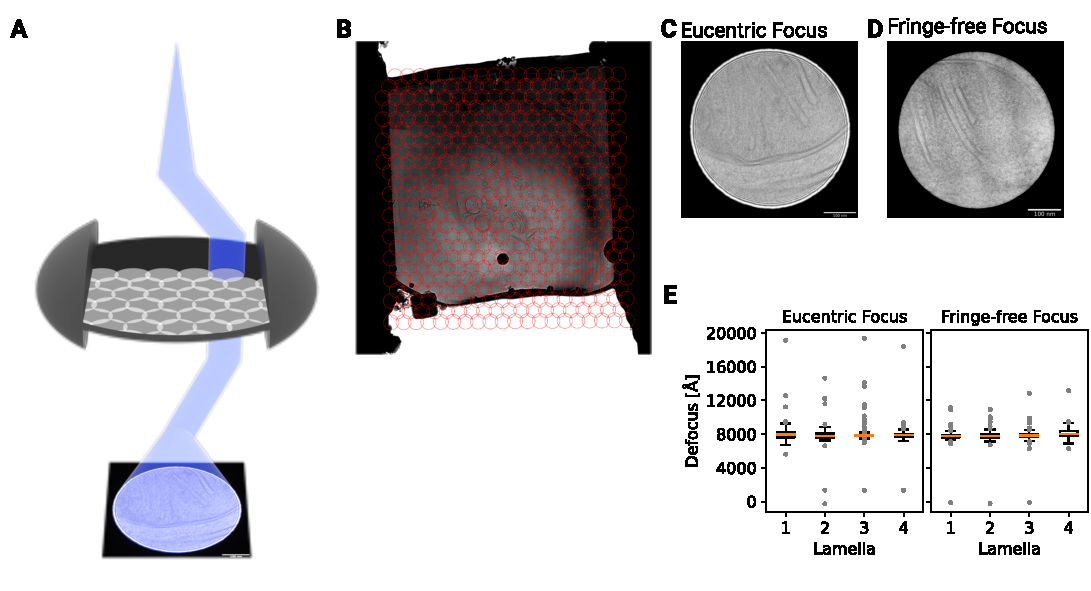
\includegraphics{figures/example-figure.pdf}
\caption{This is an example-figurern}
\end{figure}

\end{fignos:no-prefix-figure-caption}

\hypertarget{references}{%
\subsection{References}\label{references}}

\hypertarget{refs}{}
\begin{CSLReferences}{0}{0}
\leavevmode\vadjust pre{\hypertarget{ref-1B9Vt9eYu}{}}%
\CSLLeftMargin{1. }
\CSLRightInline{\textbf{Inhibition of Dihydroorotate Dehydrogenase Overcomes Differentiation Blockade in Acute Myeloid Leukemia}
\CSLBlock{David B Sykes, Youmna S Kfoury, François E Mercier, Mathias J Wawer, Jason M Law, Mark K Haynes, Timothy A Lewis, Amir Schajnovitz, Esha Jain, Dongjun Lee, \ldots{} David T Scadden} \emph{Cell} (2016-09) \url{https://doi.org/f3r5jr}
\CSLBlock{DOI: \href{https://doi.org/10.1016/j.cell.2016.08.057}{10.1016/j.cell.2016.08.057} · PMID: \href{https://www.ncbi.nlm.nih.gov/pubmed/27641501}{27641501} · PMCID: \href{https://www.ncbi.nlm.nih.gov/pmc/articles/PMC7360335}{PMC7360335}}}

\end{CSLReferences}

\end{document}
